\section{Motivation}
\label{sec:Motivation}

Given the importance of dealing with API evolution, much research has been devoted into this area. Espinha et al. \cite{espinha_web_2014} investigated the challenges for client developers regarding API changes and identified how large providers organize their evolutionary process. In \cite{brito_you_2020}, Brito et al. conducted a field study to determine the motivation of API providers to introduce breaking changes. For a better understanding of Web API evolution, Li et al. \cite{li_how_2013} examined large popular Web APIs and defined common characteristics of changes. Given the recurring features of API changes, Lübke et al. \cite{lubke_interface_2019} extracted a number of patterns for evolving Web APIs from best practices found in major public services as well as in literature. 

Due to the fact that adapting a client application to the latest version of an API is cumbersome, various approaches to automate the migration process have been proposed. However, automation techniques for library evolution such as capturing and replaying refactoring steps \cite{henkel_catchup!_2005} or using twinning to adapt to alternative APIs \cite{nita_using_2010} have been rarely adopted in practice \cite[p. 300]{li_how_2013} and cannot be applied to remote Web APIs. Although tools were created to allow developers to parse IDLs to generate client libraries and server stubs in all modern programming languages, this generated code is a static view of an API and does not support migratory adaptions. Hence, every breaking change is directly reflected in the generated library and breaks the client application. 

Regardless of whether an IDL generator is used to create a library, the workflow remains inconvenient for API consumers. Due to the independent release cycles, API providers update their code and documents without knowing how it might affect their consumers. Breaking changes are not necessarily limited to modifications to the public interface, but can also occur in the event of alterations in internal behavior such as changing standard parameters or return values. As shown in Figure \ref{fig:oldWorkflow}, API consumers may not be notified of a new release and will only find out about it after their application has malfunctioned. 

\begin{figure}[h]
	\centering{
		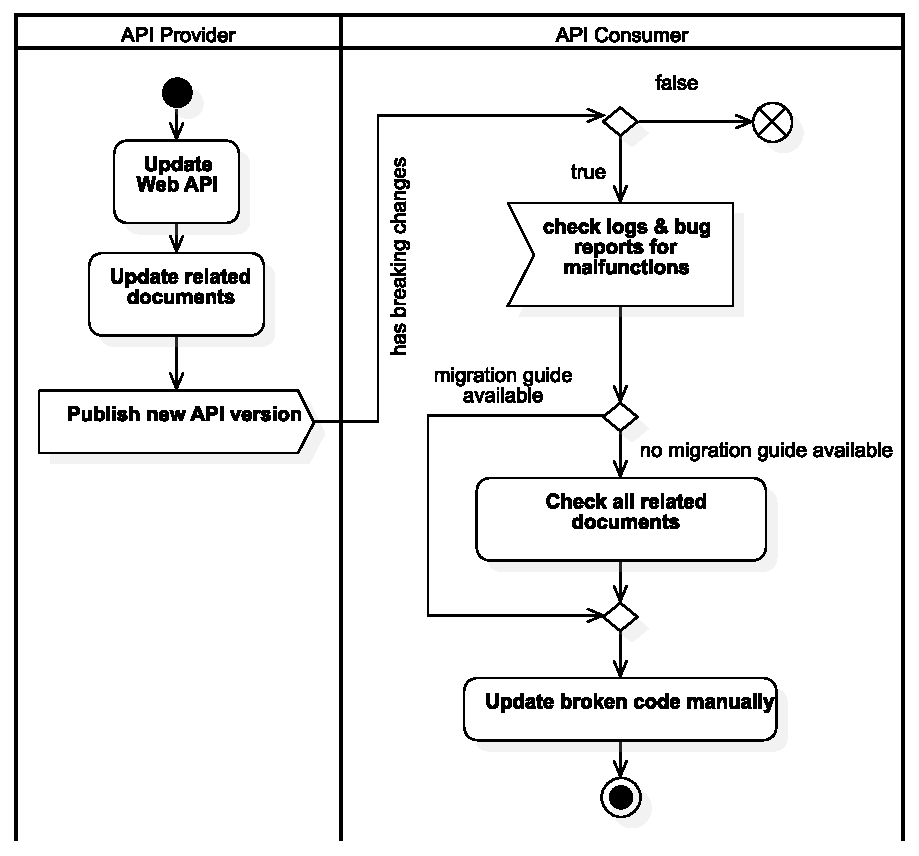
\includegraphics[width=125mm]{images/old_workflow.pdf}
		\caption{Cumbersome workflow after web service changes}
		\label{fig:oldWorkflow}
	}
\end{figure}

In a field study, Brito et. al questioned API providers on how they plan to document their changes. They found out that 22\% usually use release notes or changelogs, while only 11\% aim to provide a migration guide. Without a detailed guide that includes all of the steps required to migrate between versions, API consumers have to go through various documents and apply the modifications themselves. Resolving breaking changes manually is error-prone and leads to rising maintenance costs. A tool-based workflow could significantly shorten the time from detection to the incorporation of changes and thus reduce maintenance costs and errors.

Recent research on API evolution focuses on classifying breaking changes and patterns for Web APIs or adapting client code after updating a local library. Currently, there is a research gap regarding tool-supported workflows for migrating client applications after a Web API introduced breaking changes. Research and tools on Web API evolution have the potential to reduce development and maintenance time, improve quality and reliability of client code and prevent manually introduced bugs during the upgrade process. Automated code migration for API consumers would eliminate the need to manually inspect changes listed in change logs, newsletters, release notes or documentations and adapting the code accordingly. 